\chapter{Методология и окружение}\label{ch:chMethod}
\section{Целевая платформа}


Для проведения исследований был выбран широко используемый сервер ARM64 с архитектурой ARM V8.2-A \cite{reid2016trustworthy,xia2021kunpeng}, который имеет ближайшего конкурента - Ampere Altra Server \cite{cha2021ampere}. Исследуемая модель процессора изготовлена с использованием 7-нанометрового техпроцесса, имеет 64 ядра с тактовой частотой 2.6 ГГц. Модель включает в себя  ряд аппаратных ускорителей, в том числе криптографии (MD5, HMAC, CMAC, AES, DES/3DES,  SHA1, SHA2) и  алгоритмов сжатия (GZIP, LZS, LZ4). 

Каждый чип состоит из двух вычислительных кристаллов (SCCL) и одного кристалл интерфейса (SICL) (отсутствует на рисунке) (Рисунок \ref{chip1}). Каждый вычислительный кристалл содержит 8 кластеров центрального процессора (CCL). В свою очередь кластер центрального процессора состоит из 4х вычислительных ядер, 4х блоков кэгширования первого уровня (64К для данных и 64К для инструкций), 4х блоков кэшировния второго уровня и блока тэгов для кэша третьего уровня. Кэш третьего уровня располагается отдельно внутри вычислительного кристалла, присоединенный к общей шине, в нем также могут храниться данный из других вычислительных кристаллов. Каждое ядро представляет собой 4-х канальный суперскалярный модуль с возможностью нарушения порядка исполнения (superscalar, out-of-order).

Следует отметить, что размер кэш-линии третьего уровня исследуемого процессора составляет 128 байт, что в два раза больше размера кэш-линий более низкого уровня или кэш-линий процессоров конкурентов. 

\begin{figure}[htbp]
	\centering
	\includesvg[width = 300pt, inkscapelatex=false ]{SVG/wikichip1.drawio.svg}
	\caption{Схема целевого чипа}
	\label{chip1}
\end{figure}

Поддерживаемые расширения:
\begin{itemize}
	\item  \textbf{NEON} - Векторное расширение ARMv8
	\item  \textbf{CRC32} - Расширение для быстрого подсчета чек-суммы CRC32
	\item  \textbf{Crypto} - Криптография
	\item  \textbf{FP16} - Числа с плавающей точкой половинной точности
	\item  \textbf{RAS} -  Надежность, доступность и удобство обслуживания. (Reliability, Availability, and Serviceability)
\end{itemize}

\section{Тесты производительности}
\subsection{SPEC 2017}
В проведенном исследовании использовались два набора тестов: SPECcpu 2017 \cite{bucek2018spec} и CPUBench \cite{lu2023cpubench}. 

SPEC cpu 2017 - набор тестов для оценки производительности вычислительных систем. Существует два поднабора: целочисленный и набор тестов с плавающей арифметикой. Большая часть теуккущего исследования сосредоточена на улучшение производительности тестов с целочисленной арифметикой, однако некоторые общие соображения также применимы и к программам, использующим вычисления с плавающей точкой. Считается, что набор тестов SPEC CPU является совремнного рынка вычислений, по этому многие компании при покупке вычислительных систем сравнивают производительность с использованием именно этого набора тестов. \cite{bucek2018spec}

Набор приложений, входящих в пакет SPEC INT 2017:
\begin{itemize}
		\item  \textbf{perlbench}:  Интерпретатор языка Perl, из которого было удалено большинство особенностей, связанных с операционными системами. Включает в себя набор тестов, которые измеряют время выполнения различных операций в Perl \cite{siever1998perl}.
		\item  \textbf{gcc}: Известный компилятор языков С/C++/Fortran из коллекции компиляторов GNU \cite{gough2004introduction}. 
		\item  \textbf{mcf}: Моделирует задачу коммивояжера, где необходимо найти оптимальный маршрут для распространения товаров в различных городах, минимизируя расстояние и время пути \cite{lobel1999solving}.
		\item  \textbf{omnetpp}: OMNeT++ моделирует производительность  сети, используя алгоритмы и структуры данных для симуляции различных сценариев, таких как передача данных, маршрутизация и управление трафиком \cite{varga2019practical}.
		\item  \textbf{xalancbmk}: Моделирует производительность преобразования XML-документов в HTML- или другие XML-документы с использованием языка XSLT (XSL Transformations) \cite{euzenat2002xml}.
		\item  \textbf{x264}: Свободная и открытая библиотека для кодирования видео, которая обеспечивает высококачественное и быстрое кодирование видео в формате H.264 (MPEG-4 AVC) \cite{merritt2006x264}.
		\item  \textbf{deepsjeng}: Искусственный интеллект игры в шахматы, имеет больше 2600 ELO  \cite{sandin2021ssdf}.
		\item  \textbf{leela}: Алгоритм игры в GO, включающий оценку позиции на основе метода Монте-Карло, выборочный поиск по дереву на основе верхних доверительных границ и оценку хода на основе рейтингов ELO \cite{choi2022does} .
		\item  \textbf{exchange2}: Программа, разработанная для генерации нестандартных и сложных судоку. Использовался на неофициальных соревнованиях, которые могли длиться несколько дней \cite{10.1145/1124708.1124709}. 
		\item  \textbf{xz}: Содержит компрессионный и декомпрессионный алгоритмы \cite{koranne2011compression}. 
\end{itemize}

В наборе тестов SPEC существует два основных типа замера - speed и rate. В режиме speed разрешается использовать оптимизации с профилем, опции для каждого теста могут подбираться индивидульно. Однако в данной диссертации используется режим rate, в котором набор опций для всех тестов должен быть унифицирован и использование профиля запрещено. Запуск возможен как в режиме  одной копии - ресурсы машины доступны одному процессу полностью, так и  в режиме множество копий, в котором процессам приходится делить общие ресурсы, такие как шину памяти или кэши. Стоит отметить, что ни в каком из наборов нельзя использовать прямо или косвенно информацию, специфичную для конкретных тестов. Так, например, в 2024 году более 2000 результатов  были помечены, как использующие информацию о тестах, а значит нечестные \cite{cliffFlagged}.

\subsection{CPUBench}

В 2023 году Китайский институт электроники и стандартизации выпустил новый набор тестов производительности для вычислительных систем \cite{lu2023cpubench}. В отличие от набора spec, CPUBench разработан на языке python и имеет в себе тесты, написанные на языке java. Авторами утверждается, что данный набор тестов является своеобразным расширением spec 2017, которое нацелено на лучшее покрытие мирового рынка (в том числе китайского). Было продемонстрировано на 14 различных платформах, что данный набор тестов сохраняет корреляцию производительности, показываемую пакетом spec.

Целочисленный набор состоит из следующих тестов:
\begin{itemize}
	\item  \textbf{x264, gcc, xz}: Схожие с пакетом spec int 2017, отличаются наборами входных данных и версиями приложений.
	\item  \textbf{gzip}: Архиватор, использующий алгоритм LZMA2 \cite{akoguz2016comparison}.
	\item  \textbf{tpcc}: Бенчмарк, который моделирует  деятельность розничного дистрибьютора с большим количеством складов и клиентов \cite{leutenegger1993modeling}.
	\item  \textbf{tpch}: Еще одна база данных, однако эта состоит набора бизнес-ориентированных запросов и модификаций данных. Иллюстрируется система принятия решений \cite{barata2015overview}.
	\item  \textbf{kmeans}: Java тест, решающий задачу K-ближайших соседей.
	\item  \textbf{wordcount}: Java тест, подсчитывающий количество слов в больших файлах. 
	\item  \textbf{velvet}: Пакет алгоритмов, разработанный для сборки генома и выравнивания секвенирования коротких считываний \cite{zerbino2008velvet}. 
	\item  \textbf{openssl}: Криптографический инструментарий, реализующий различные алгоритмы шифрования \cite{rescorla2001introduction}.
	\item  \textbf{rapidjson}: Библиотека для парсинга Json -файлов\cite{keiser2023demand}
	\item  \textbf{python}: Интерпретатор языка Python \cite{python2021python}.
\end{itemize}


Можно заметить некоторую схожесть с пакетом SPEC int. Так вместо интерпретатора языка perl представлен интерпретатор более современного языка python, добавлен дополнительный алгоритм компрессии/декомпрессии, парсинг XML документов заменен на парсер JSON файлов. А вот алгоритмов искусственного интеллекта здесь не наблюдается, зато присутствую базы данных MySQL и криптографический инструмент openssl.

\section{Методология измерения}
В данной диссертаций используется измерения типа  SPECrate base и ее аналог typcal в CPUBench. В данной методологии предусмотрены следующие шаги:
\begin{enumerate} 
		\item Измерение времени выполнения каждого теста, запущенного в $NUM\_COPIES$ копий, в некоторое количество итераций ($N$)
		\item Если было запущено больше одной копии, то временем исполнения теста считается самое большое время среди всех копий.
		\item Для каждого теста выбирается медианное время среди проделанных итераций. 
		\item Обратное медианное время каждого теста умножается на референсное время ($REF\_TIME$), полученное на фиксированной машине. Например, для SPEC 2017  это  Sun Fire V490 with 2100 MHz UltraSPARC-IV+.
		\item Считается среднее геометрическое по всем тестам. Использование среднего геометрического обосновывается свойством сохранения отношения.
		\item Полученное число умножается на количество копий.
\end{enumerate}
Если всего в сете $M$ тестов, то кратко можно записать формулу расчета производительности следующим образом:

$$RATE =\left(\prod _{i=1}^{M}\dfrac{REF\_TIME_i}{MEDIAN(TIME_{i1}, TIME_{i2}, ... , TIME_{iN})}\right)^{\frac {1}{M}} $$

Также важной частью считается настройка окружающей системы, направленная на уменьшение флуктуаций времени исполнения тестов и лучшей утилизации тестовой системы.
Так как эта тема не является прямой темой данного исследования, а лишь косвенного затрагивает ее, но тем не менее весьма важна, ниже предлагается ознакомится с проблемами, которыми пришлось столкнуться во  время проведения замеров для алгоритмов реализованных в данной диссертации.  

\begin{itemize}
	\item  \textbf{Троттлинг} - технология изменения частоты процессора при превышении критических температур. Часто возникает при нарушении системы охлаждения или неправильной эксплуатации. Проявляется в виде увеличения времени исполнения теста с каждой следующей итерацией \cite{zhang2009hardware}.
		\begin{figure}[ht]
		\centerfloat{
			\includegraphics[scale=1]{PNG/ddr1}
		}
		\caption{Схема подсистемы памяти целевой платформы.}\label{fig:ddrsvg1}
	\end{figure}
	\item  \textbf{Неполная утилизация ресурсов системы} - Целевая платформа имеет восемь каналов DRAM, с возможностью подключения до двух плашек на каждый канал (Рисунок \ref{fig:ddrsvg1}). В случае, если какой-то канал остался незадействованным (Например, воткнуты подряд, а не через одну) то будет наблюдаться картина, как на рисунке \ref{fig:lack_of_memmory}. Можно видеть, что неиспользуемые порты приводят к томму, что вычислительным ядрам приходится обращаться за ресурсами памяти в соседние блоки, что значительно замедляет исполнение.

	
	\begin{figure}[ht]
		\centerfloat{
			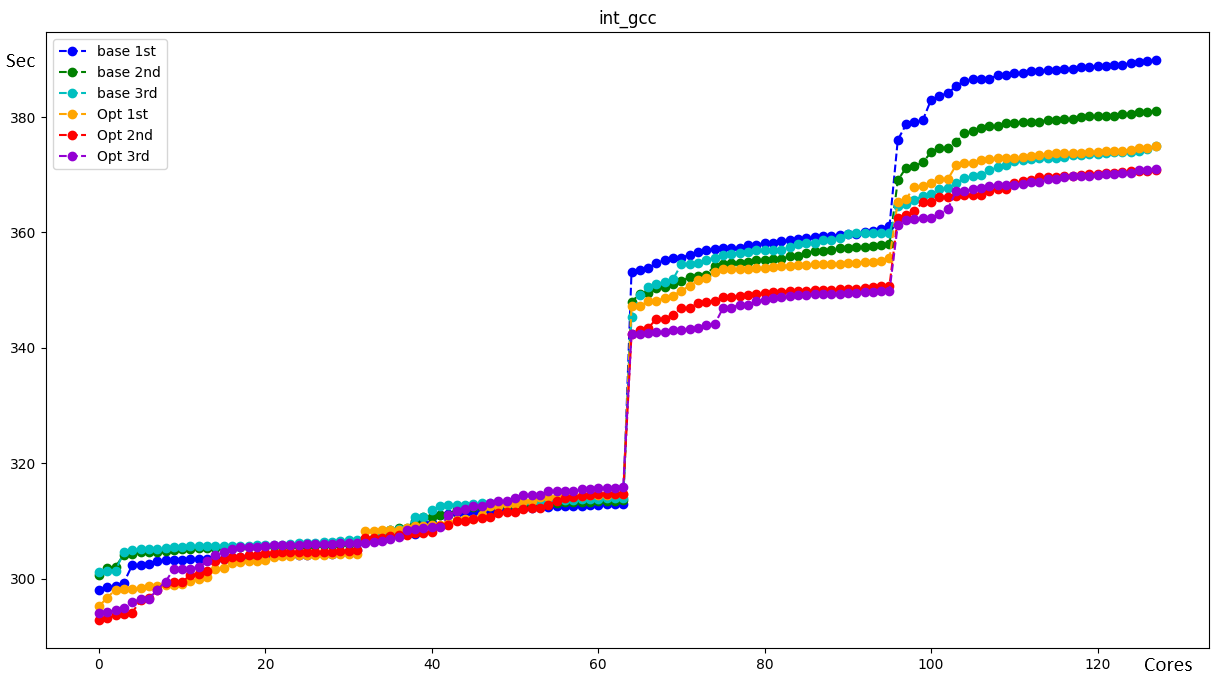
\includegraphics[scale=0.5]{PNG/lack_of_memmory}
		}
		\caption{Зависимость времени исполнения приложения от номера ядра при неправильном подключении плашек оперативной памяти.}\label{fig:lack_of_memmory}
	\end{figure}
	\item \textbf{Рандомизация размещения адрессного пространства (ASLR)} - Технология, изначально разрабатываемая для защиты процессов от различного рода атак с использованием  переполнения буфера. При этом  адреса расположения исполняемого файла рандомизируются для усложнения предсказания положения объекта в памяти и получения доступа из сторонних процессов \cite{gras2017aslr}. Однако в случае аккуратных измерений производительности системы эта технология может приводить к случайному наложению младших частей адресов и соответственно попаданию в одну и ту же кеш линию. На рисунке \ref{fig:peaks}  можно видеть как на случайном ядре время исполнения отдельной копии увеличивается больше чем в 2 раза.
	\item \textbf{Частота обновления оперативной памяти} - Оперативная память, являясь энергозависимой памятью требует постоянного обновления значений в ячейках. Частота обновления этих ячеек регулируется в BIOS. С одной стороны большая частота обновления уменьшает количество ошибок и связанных с ними задержек, однако с другой стороны обновление памяти это по своей сути дополнительная загрузка данных, что в высоко нагруженной системе может создавать дополнительные задержки. По-этому этот параметр приходится подбирать эмпирическим путем, и он оказывает существенное влияние на итоговую производительность системы.
	
	\begin{figure}[ht]
		\centerfloat{
			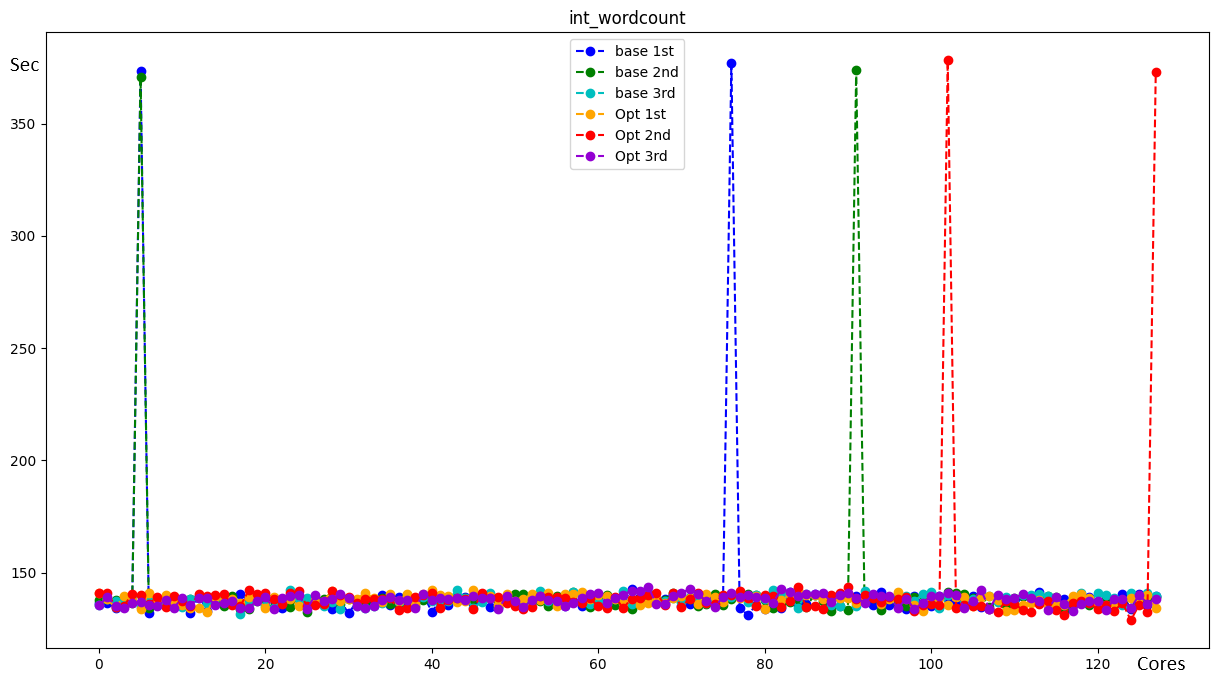
\includegraphics[scale=0.5]{PNG/peaks}
		}
		\caption{Зависимость времени исполнения приложения от номера ядра при замере c включенной ASLR.}\label{fig:peaks}
	\end{figure}
	\item \textbf{Занятость ресурсов внешними программами} - Достаточно очевидный факт: если необходимо измерить производительность системы, то ваш бенчамрк должен быть единственным, исполняемым на этой системе.  Однако организовать тест в вакууме достаточно сложно, так как операционная система время от времени может запускать демонов, планировщик и прочее,  методы борьбы с этим индивидуальны и не будут указаны здесь, однако, покажем, как пронаблюдать этот эффект. Если мы производим высокоинтенсивной замер, утилизирующий все ядра и большинство остальных ресурсов системы, а затем отсортируем время выполнения тестов на разных ядрах, то можем получить картину, как на рисунке \ref{fig:tails}. Эти "хвосты" чаще высего означают, что система была занята другими  приложениями, а не  тестом.
\end{itemize}


\begin{figure}[ht]
	\centerfloat{
		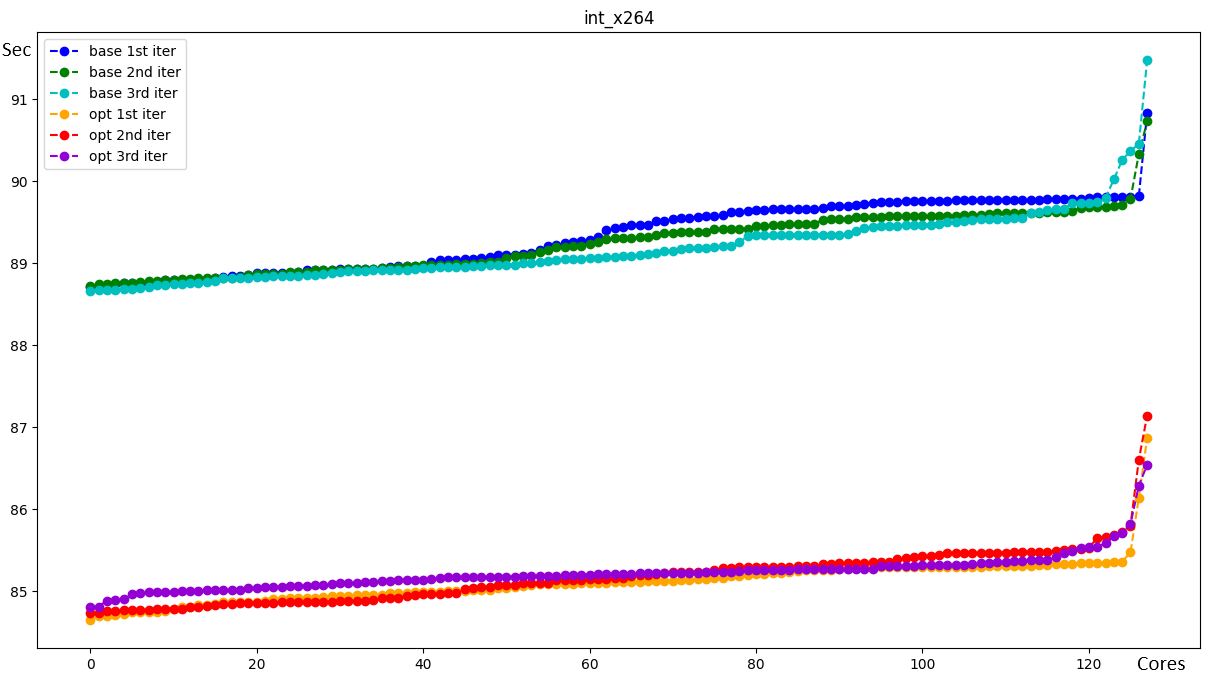
\includegraphics[scale=0.5]{PNG/tails}
	}
	\caption{Зависимость времени исполнения приложения от номера ядра при замере на загруженной системе.}\label{fig:tails}
\end{figure}



Приведенные проблемы нельзя решить после замера каким-либо "обрезанием хвостов" или "удалением пиков" из выборки. Методология такого не позволят. Если бы подобные манипуляции были возможно, то это позволило бы вендорам манипулировать данными, ведь тогда пришлось бы вводить какие-либо правила, когда и как можно корректировать данные замеров, что привело бы к махинациям ради получения более высоких цифр производительности.

\section {Профилирование}

